\documentclass{article}
\usepackage{graphicx}
\usepackage{float}
\usepackage{amssymb}

\title{Manual do Sintetizador}
\author{Guido Stolfi}
\date{19/DEZ/1974}

\begin{document}
\maketitle

\section{OBSERVAÇÕES}
\subsection{}
Os potenciômetros da fileira de cima e os dois primeiros à esquerda da fileira de baixo estão ligados entre terra e +5Volts sendo acessível apenas o "tap". (v. pg. 63 e 47)

\subsection{}
Os multiplicadores da esquerda, metade superior, (com bornes c amarelos ao invés de verdes), estão ligados como FILTROS com frequência de corte descrita na pg. 43

\subsection{}
Consumo típico:

\begin{tabular}{r|r}
fonte de 5Volts & ~4,5A \\
\hline
+15Volts & 0,15A \\
\hline
-15Volts & 0,15A \\
\end{tabular}

Importante: Ajustar a tensão +5 para obter +5,00 Volts entre os bornes +5 (amarelos) e terra (pretos) no painel dos potenciometros, o que corresponde a quase 5,4 Volts nos bornes da fonte regulada.

\subsection{}
Os conversores D/A estão ligados para faixa de 0V (entrada 0000 0000) a +5Volts (entrada 1111 1111)

\subsection{}
Falta ligar fonte de -5Volts (fio verde) se for preciso.


\section{Módulo gerador de timbres}
Este é essencialmente um conversor D/A PCM de 16 níveis e 32 bits (por período). Produz na sua saída uma forma de onda ímpar de freqüência 32 vêzes menos que a da referência.

\begin{figure}
\centering
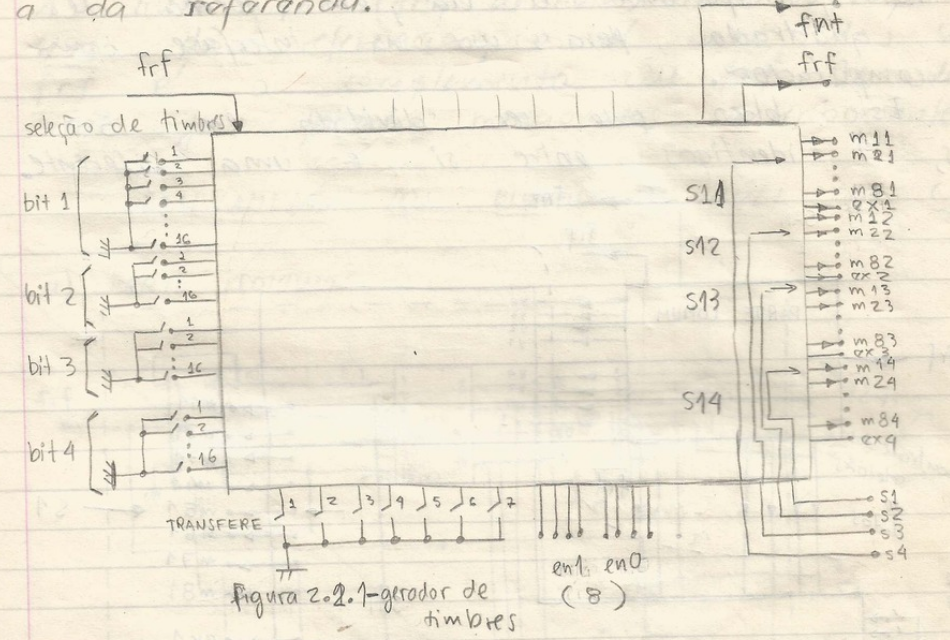
\includegraphics[width=12cm]{figuras/2.2.1-gerador de timbres.png}
\caption{gerador de timbres}
\end{figure}

Todos os sinais são digitais. \textit{frf} é a freqüência de referência, 32 vezes maior que a da nota a ser executada. Um timbre pode ser selecionado pelos 4 grupos de 16 chaves de seleçao de timbres. Um timbre programado manualmente nesta entrada pode ser transferido (manualmente) para uma de 7 memórias (numeradas de 1 a 7) pelos comandos \textit{TRANSFERE}. As entradas \textit{en\textsubscript{0}} e \textit{en\textsubscript{1}} são entradas série de "1" e "0" para a 8.a memória, a ser usada pelo computador. A saída m\textsubscript{ij} (j = 1, 2, 3, 4) executa o timbre armazenado na i-ésima memória (i = 1,2,...,8), em quatro linhas de informação digital, a ser convertida por um conversor D/A de 4 bits na forma de onda desejada. Além destas temos também a saída ex\textsubscript{1}, ex\textsubscript{2}, ex\textsubscript{2} e ex\textsubscript{4}, correspondente ao timbre selecionado externamente (chaves de seleção).

Qualquer destas saídas pode ser selecionada pela chave S1 de 9 posições 4 polos, sendo disponível na saída s\textsubscript{1}, s\textsubscript{2}, s\textsubscript{3} e s\textsubscript{4}.

As saídas frf e fnt são respectivamente na freq. de referência de entrada e na frequência da nota correspondente a ela, em forma de onda quadrada, para uso na interface com o computador.

Este bloco pode ser dividido em 5 partes, 4 identicas entre si e uma diferente.

\begin{figure}[H]
\label{detalhamento do gerador de timbres}
\centering
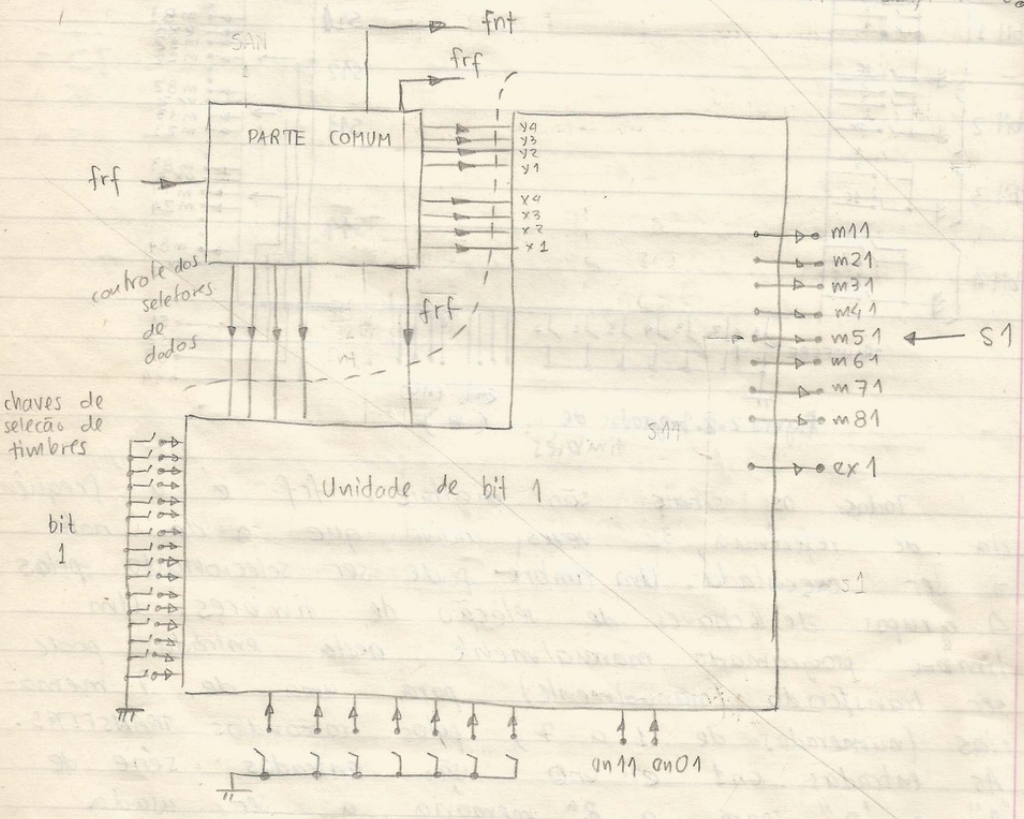
\includegraphics[width=12cm]{figuras/2.2.2-detalhamento do gerador de timbres.png}
\caption{detalhamento do gerador de timbres}
\end{figure}

Na figura \ref{detalhamento do gerador de timbres} temos um detalhamento do gerador de timbres contendo a parte comum e uma das 4 partes idênticas (correspondente ao bit 1). A parte comum compreende divisores de freqüência até 32, e decodificadores que devem gerar os sinais x e y de controle das unidades de bit 1, 2, 3 e 4. As quatro linhas de controle dos seletores de dados conduzem sinais de freqüência 1/2, 1/4, 1/8 e 1/16 da freqüência de referência de entrada. A linha fnt (freq. de nota) tem freqüência 1/32 da referência, e é uma das saídas. $\overline{frf}$ é o complemento de frf. Os demais sinais já foram mencionados anteriormente.

\subsection{DETALHAMENTO DOS BLOCOS EM NÍVEL DE C.I.}

\subsubsection{(a) PARTE COMUM}
\begin{figure}[H]
\centering
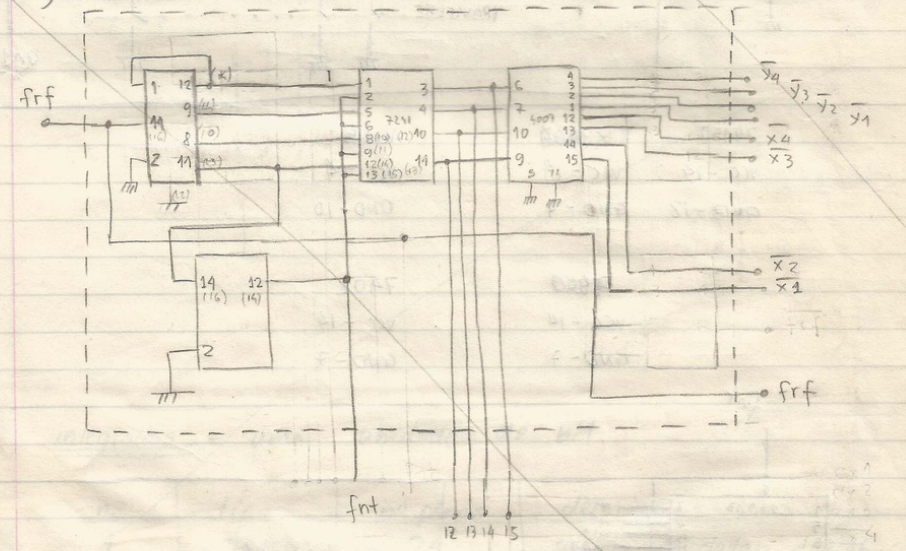
\includegraphics[width=12cm]{figuras/detalhamento dos blocos em nivel de ci - parte comum.png}
\end{figure}


\subsubsection{(b) UNIDADES DE BIT 1, 2, 3, 4}
\begin{figure}[H]
\centering
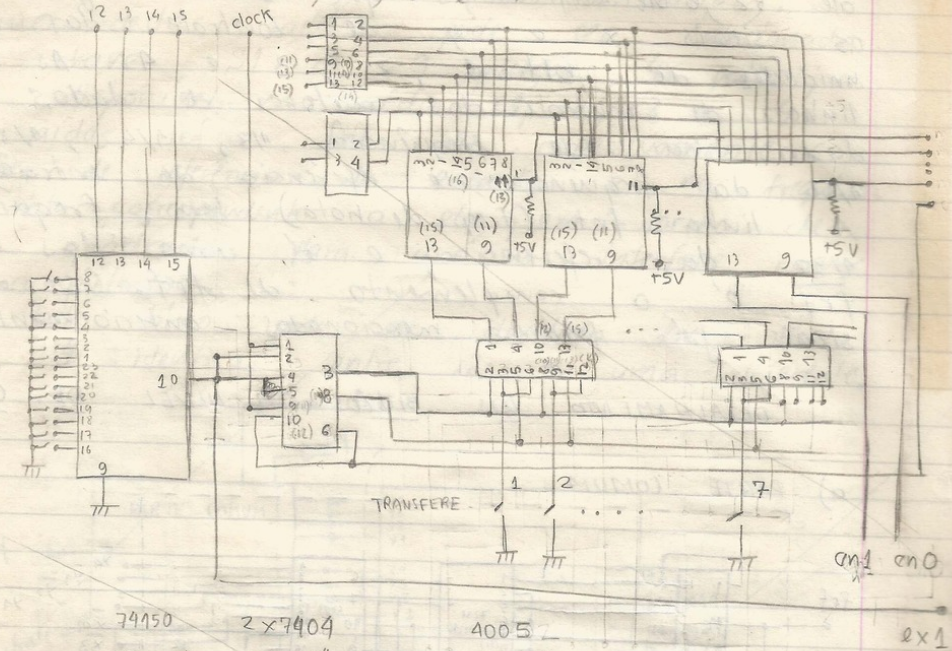
\includegraphics[width=12cm]{figuras/detalhamento dos blocos em nivel de ci - unidades de bit 1, 2, 3 e 4.png}
\end{figure}

\begin{tabular}{c c c}
74150 & 2 x 7404 & 4005 \\
VCC - 14 & VCC - 14 & VCC - 4 \\
GND - 12 & GND - 7 & GND - 10 \\
 & & \\
 & 7400 & 7402 \\
 & VCC - 14 &  VCC - 14 \\
 & GND - 7 &  GND - 7 \\
\end{tabular}

\begin{figure}[H]
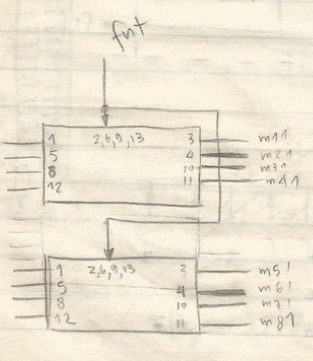
\includegraphics[width=5cm]{figuras/detalhamento dos blocos em nivel de ci - unidades de bit 1, 2, 3 e 4 - parte 2.png}
\end{figure}

\begin{tabular}{c c c}
3 x 7241 \\
VCC - 14 \\
GND - 7 \\
\end{tabular}

\subsubsection{(c) Formas de onda}
(figura se soltou do caderno. Será que está em algum outro lugar?)

\subsubsection{integrados - uma unidade de bit}

\begin{tabular}{|c|c|c|c|}
\hline
n.o & tipo & n.o pinos & descrição \\
\hline
1 & 74150 & 24 & seletor de dados de 16 canais \\
8 & 4005 & 14 & memória de 16 bits \\
2 & 7404 & 14 & hex-inversor \\
3 & 7241 & 14 & quádruplo ou-exclusivo \\
4 & 7402 & 14 & nor quádruplo \\
\hline
\end{tabular}

\subsubsection{entradas - uma unidade de bit}

\begin{tabular}{|c|c|}
\hline
n.o & sinal (sinais) \\
\hline
1 & frf \\
4 & controle do seletor de dados \\
8 & dos decodificadores \\
16 & chaves de entrada \\
7 & chaves de transferência \\
1 & en\textsubscript{1} \\
1 & en\textsubscript{0} \\
\hline
38 & \\
\hline
\end{tabular}

\subsubsection{saídas}

\begin{tabular}{|c|c|}
\hline
n.o & sinal (sinais) \\
\hline
8 & m\textsubscript{ij} * \\
1 & e\textsubscript{xi} * \\
\hline
\end{tabular}

Alimentação:
- TERRA
- +5V

\subsection{PARTE COMUM}

ENTRADAS:

\begin{tabular}{c|c}
n.o & sinal \\
\hline
1 & frf \\
\end{tabular}


SAÍDAS:

\begin{tabular}{c|l}
n.o & sinal \\
\hline
1 & frf * \\
1 & fnt * \\
8 & dos decodificadores \\
4 & para os seletores de dados \\
\end{tabular}


\subsection{OBSERVAÇÃO IMPORTANTE}
Mostrou-se mais insteressante particionar o gerador de timbres de maneira diferente da até agora usada. Assim, a partição anteriormente feita fica a partir de agora abandonada.

\subsection{Diagrama funcional:}
(caderno escaneado não tem esse desenho. Está guardado solto em algum lugar?)


\subsection{Cartão da parte comum:}
(IMAGEM)

\subsection{Cartão de unidade de memória:}
(IMAGEM)

(TABELA: "Interligações com cartão da parte comum:")

\section{VIBRATO:}
(IMAGEM)

\section{TECLADO:}
(IMAGEM)

\subsection{ENTRADA DO TECLADO (PARTE COMUM)}
(IMAGEM)
(IMAGEM)

Filtro controlado por tensão.
(IMAGEM)

Filtro controlado por tensão.
(IMAGEM)

Conversor freqüência-tensão
(IMAGEM)

Gerador de envoltória - controle de tempo de subida, tempo de descida e duração por potenciômetros
controle de tensão máxima, mínima e duração (opcional) por tensão
(IMAGEM)

Mono 1 - dispara na subida
Mono 2 - dispara na subida
S1 - conduz quando C1 = 1
S2 - conduz quando C2 = 1
S3 - 1 - duração controlada externamente
     2 - duração controlada por chv
(IMAGEM)
(IMAGEM)

\section{NOVA MUDANÇA De PLANOS}

Aqui resolveu-se optar por uma solução log-exp para os blocos do sintetizador. Assim, em principio todas entradas são para o logaritmo da que era entrada anteriormente. Assim, um VCO pode ser representado assim:

a) VCO
(IMAGEM)

valores para k1 e k2 para se obter f = frf seriam:

(...)

b) Um filtro controlado por tensão fica sendo

(...)
(IMAGEM)

c) Multiplicador
(IMAGEM)
(IMAGEM)

V.C.O. CIRCUITO PROPOSTO
(IMAGEM)

\section{GERADOR DE ENVOLTORIAS}
(IMAGEM)

\subsection{GERADOR DE ENVOLTORIA:}
objetivo: gerar forma de onda trapezoidal de 0 a +5V, com os seguintes parâmetros controlados:

portensão:

1 -> tempo de subida ~ de 3ms a 30s;
2 -> tempo de queda ~ de 3ms a 30s;
3 -> tempo de duração (modo A) ~3ms a 30s;


digitais:
1 -> início da subida;
2 -> início da queda (modo B);
3 -> indicação MODO A - MODO B <- SELECIONOAVEL P/ COMPUTADOR DIRETAMENTE

(IMAGEM)

\section{INTERFACE RECEPTORA}
(IMAGEM)
(IMAGEM)

\subsection{FORMAS DE ONDA NA INTERFACE RECEPTORA}
(IMAGEM)

\subsection{INTERFACE DE NOTA}
(IMAGEM)

\subsection{V.C.F.}
(IMAGEM)

\section{Descrição de um sintetizador de som modular}
\subsection{Introdução}
Este sintetizador é composto de módulos ou blocos funcionais que executam funções simples. As entradas dos blocos podem ser analógicos ou digitais. As entradas analógicas são para tensões de 0 a 5 volts (sinais monopolares) ou de -5 a +5 volts.
As entradas digitais são em nível de lógica TTL. As saídas dos blocos também podem ser digitais ou analógicas, seguindo o mesmo critério das entradas.

Em princípio, qualquer saída analógica pode ser ligada a uma entrada analógica.

Qualquer saída digital pode ser ligada a uma entrada digital. As saídas analógicas de 0 a +5 volts podem ser ligadas a entradas digitais.

Para que todas as grandezas possam ser controladas numa faixa dinamica de 3 décadas, mostrou-se conveniente uma lei exponencial de controle para certas funções conforme se verá posteriormente.

O sintetizador tem a possibilidade de executar uma nota musical de cada vez constituindo-se, portanto, num instrumento monofônico. Interligando-se convenientemente os blocos, pode-se controlar muitos parâmetros da nota musical executada como altura, intensidade, timbre, formante, portamento, vibrato, envoltórias, trêmolo, etc.

Composições polifônicas podem ser obtidas por superposição de melodias monofônicas através de regravações sincronizadas, em fita magnética.

Os controles dos blocos podem ser feitos manualmente através de teclados, chaves potenciometros e pedais, ou automaticamente usando um computador.

\subsection{Descrição dos blocos funcionais}
\subsubsection{Teclado (TECL)}

O teclado tem a função de produzir os seguintes sinais de saída:

a) Frequencia de referencia - frf

Onda quadrada (digital) de frequencia selecionavel entre 121 (manualmente) ou 120 (automaticamente), valores 32 vezes maiores que as das notas musicais, a saber, do dó de 1635 Hz e 16744,0 Hz na posição manual e do de 16,35 Hz a si de 15804,3Hz na posição automático. Todas as oitavas são justas, havendo 12 geradores independentes que podem ser afinados em qualquer escala de 12 notas.

b) Controle de chaveamento - CHV

Sinal analógico que assume o valor 0 Volts se nenhuma tecla do manual é acionada, e 5 volts em caso contrario (na posicao manual). Na posicao automatico, o sinal de chaveamento é designado por comando especifico (0 volts para "nota silenciosa" e 5 volts para "nota").

C) controle de inicio de nota - L -
pulso estreito de 5 volts a cada acionamento de qualquer tecla.

c') fim de nota (D) idem a L, no desacionamento de cada nota. As entradas são:

d) controle de vibrato - VBR
Sinal analógico (-5Volts a +5Volts) que provoca um desvio relativo na frequência f da nota executada segundo a relação:

(MATH)

e) "strobe" e dados relativos a nota (frf) e ao chaveamento (CHV) - sinais digitais para comando automatico do teclado.

Os controles manuais são:

f) manual de 49 teclas

g) chave de 7 posicoes para transposição de oitavas.

3. Chave manual-automático
(IMAGEM)

\section{Circuito de portamento (PORT)}
(IMAGEM)
(...) 
\section{Gerador de timbres}

Esse bloco tem por função produzir formas de ondas (timbres) que podem ser programadas num painel gráfico ou por computador. Possui 7 memórias de armazenamento de formas de onda

\end{document}
